% !TeX program = lualatex
% !BIB program = biber
% Lualatex is important to render TTF fonts; with pdflatex it's just the regular one
% ratio 16:9 -- https://tex.stackexchange.com/questions/14336/

% compile two versions, inspired by https://tex.stackexchange.com/a/1501
% use the script "compile-pdf.sh"
\newif\ifhandout
% if flags.tex does not exist, create an empty file to be able to compile in TeXstudio
\input{flags}

\ifhandout
\documentclass[12pt,aspectratio=169,handout]{beamer}
\else
\documentclass[12pt,aspectratio=169]{beamer}
\fi



% TODO change "leftfootertext" to your liking
\newcommand{\leftfootertext}{\insertsubtitle}  % just the \title{} text by default
%\newcommand{\leftfootertext}{RNNs and encoder-decoder architectures}  % Your name, for instance


% ------- RUB specifics ----------
% adjust for 16:9
% https://tex.stackexchange.com/questions/354022/modifying-the-margins-of-all-slides-in-beamer
\setbeamersize{text margin left=0.3cm,text margin right=4.5cm} 


% use Metropolis as the basis theme
\usetheme[subsectionpage=progressbar]{metropolis}
% blocks with background globally
\metroset{block=fill}


\usepackage{fontspec}
% RUB fonts need to be installed
% 'UprightFont = * Light' makes sure that the base font is RubFlama Light, which looks
% lighter than RubFlama Regular (would be too thick for slides)
\setsansfont[Scale=MatchLowercase, UprightFont = * Light, BoldFont = * Bold]{RubFlama}
%\setsansfont{Arial} % Open source alternative if you don't have RubFlama

% RUB color scheme
% Dark blue: 0; 53; 96; #003560
\definecolor{RUBDarkBlue}{RGB}{0, 53, 96}

% Light yellow (table fill, etc.); 238; 250; 196; #EEFAC4
\definecolor{RUBLightYellow}{RGB}{238, 250, 196}

%Light green: 141; 174; 16
\definecolor{RUBLightGreen}{RGB}{141, 174, 16}


\setbeamercolor{titlelike}{fg=RUBDarkBlue}
\setbeamercolor{subtitle}{fg=RUBLightGreen}
\setbeamercolor{separation line}{fg=RUBLightGreen}
\setbeamercolor{frametitle}{bg=white, fg=RUBDarkBlue}

% horizontal line on title page and sections
\setbeamercolor{alerted text}{fg=RUBLightGreen}


% Adjust footer bottom (too large by default)
\setbeamertemplate{footline}{%
  \begin{beamercolorbox}[wd=\textwidth, sep=2ex]{footline}%
    \usebeamerfont{page number in head/foot}%
    \usebeamertemplate*{frame footer}
    \hfill%
    \usebeamertemplate*{frame numbering}
  \end{beamercolorbox}%
}


% Lab name, numbering, etc. in footer
\setbeamertemplate{frame numbering}{TrustHLT --- Prof.\ Dr.\ Ivan Habernal \hspace*{1ex} 
\includegraphics[width=7em]{img/rub-logo.pdf}\hspace*{1ex}}

\setbeamertemplate{frame footer}{\hspace*{1ex}\insertframenumber \hspace*{2ex} \leftfootertext}

% adjust the background to be completely white
\setbeamercolor{background canvas}{bg=white}

% logos on the title page
\titlegraphic{%
	\begin{picture}(0,0)
		\put(435,0){\makebox(0,0)[rt]{
\includegraphics[width=7em]{img/rub-logo.pdf}}}
		\put(435,-170){\makebox(0,0)[rt]{
\includegraphics[width=4em]{img/logo-trusthlt.pdf}}}
		\put(435,-196){\makebox(0,0)[rt]{
\includegraphics[width=9em]{img/logo-rctrust.pdf}}}
	\end{picture}%
}


% show TOC at every section start
\AtBeginSection{
	\frame{
		\vspace{2em}
		\sectionpage
		\hspace*{2.2em}\begin{minipage}{10cm}
			\tableofcontents[currentsection]
		\end{minipage}
	}
}

% TOC without subsection
\setcounter{tocdepth}{1} % only-- part,chapters,sections 

% bullet points: rectangles
\useinnertheme{rectangles}
\setbeamercolor{itemize item}{fg=RUBLightGreen}
\setbeamercolor{itemize subitem}{fg=RUBLightGreen}
% enumerate: blue background for better readability
\setbeamercolor{item projected}{bg=RUBDarkBlue}

% make boxes (example, block, etc.) background lighter for readability
\setbeamercolor{block title}{%
	use=normal text,
	fg=normal text.fg,
	bg=normal text.bg!90!fg % lighter background in block title
}
\setbeamercolor{block body}{
	use={block title, normal text},
	bg=block title.bg!30!normal text.bg % lighter background in block body
}


% RUB colors in blocks
\setbeamercolor{block title alerted}{%
	use={block title, alerted text},
	bg=RUBDarkBlue,
	%fg=RUBLightYellow % looks bad
	fg=white % better contrast
}

\setbeamercolor{block title example}{%
	use={block title, example text},
	fg=RUBLightGreen
}


% ------- end of RUB specifics ----------

% all itemize with pause by default
%\beamerdefaultoverlayspecification{<+->}


% typeset mathematics on serif
\usefonttheme[onlymath]{serif}

% better bibliography using biber as backend
\usepackage[natbib=true,backend=biber,style=authoryear-icomp,maxbibnames=30,maxcitenames=9,uniquelist=false,giveninits=true,doi=false,url=false,dashed=false,isbn=false]{biblatex}
% shared bibliography
\addbibresource{../bibliography.bib}
% disable "ibid" for repeated citations
\boolfalse{citetracker}



\usepackage{xspace}


% for derivatives, https://tex.stackexchange.com/a/412442
\usepackage{physics}

\usepackage{tikz}
\usetikzlibrary{matrix, positioning}
\usetikzlibrary{angles,quotes} % for angles
\usetikzlibrary{backgrounds} % background
\usetikzlibrary{decorations.pathreplacing} % curly braces
\usetikzlibrary{calligraphy}
\usetikzlibrary{calc} % for neural nets

% for plotting functions
\usepackage{pgfplots}
\usepgfplotslibrary{dateplot}

% sub-figures
\usepackage{caption}
\usepackage{subcaption}

% book tabs
\usepackage{booktabs}


% argmin, argmax
\usepackage{amsmath}
\DeclareMathOperator*{\argmax}{arg\!\max}
\DeclareMathOperator*{\argmin}{arg\!\min}
% softmax
\DeclareMathOperator*{\softmax}{soft\!\max}
% Mask
\DeclareMathOperator*{\mask}{mask}

% bold math
\usepackage{bm}

% for \mathclap
\usepackage{mathtools}

% algorithms
\usepackage[noend]{algpseudocode}


% for neurons and layers in tikz
\tikzset{
	neuron/.style={draw, rectangle, inner sep=2pt, minimum width=0.75cm, fill=blue!20},
	param/.style={draw, rectangle, inner sep=2pt, minimum width=0.75cm, fill=green!20},
	constant/.style={draw, rectangle, inner sep=2pt, minimum width=0.75cm, fill=black!15},
	% for citation nodes right top
	ref/.style={anchor = north east, text width=7.8cm, yshift=-1.3cm, xshift=-0.2cm, scale=0.5},
	state/.style={rectangle, inner sep=2pt, minimum width=0.75cm, fill=black!5},
}

% added in lecture 10
\tikzset{
	mtx/.style={
		matrix of math nodes,
		left delimiter={[}, right delimiter={]}
	},
	hlt/.style={opacity=0.1, line width=4 mm, line cap=round},
	hltr/.style={opacity=0.5, rounded corners=2pt, inner sep=-1pt}
}

% for strike-through text (added in Lecture 06)
\usepackage[normalem]{ulem}

% added in Lecture 7
% RNN
\DeclareMathOperator*{\rnn}{RNN}
% RNN star
\DeclareMathOperator*{\rnnstar}{RNN^{*}}
% bi-RNN
\DeclareMathOperator*{\birnn}{biRNN}


% added in Lecture 9
\usetikzlibrary{fit} % for hightligting by calling "fit"

% algorithms
\usepackage[noend]{algpseudocode}



\title{Privacy-Preserving Natural Language Processing}
\subtitle{Lecture 8 -- Applications of DP-SGD and machine unlearning}
\date{July 03, 2025}
\author{Prof.\ Dr.\ Ivan Habernal}
\institute{
\texttt{www.trusthlt.org} \\
Chair of Trustworthy Human Language Technologies (TrustHLT) \\
Ruhr University Bochum \& Research Center Trustworthy Data Science and Security}

\begin{document}


\maketitle



\section{The Obvious Application: Supervised Training}

\begin{frame}{DP-SGD across various NLP tasks}

Setup:

Although DP-SGD had been used in language modeling, the community lacked a thorough understanding of its usability across different NLP tasks

Research questions:

\begin{itemize}
\item Which models and training strategies provide the best trade-off between privacy and performance on different NLP tasks?
\item How exactly do increasing privacy requirements hurt the performance?
\end{itemize}


\begin{tikzpicture}[overlay, remember picture]
\node at (current page.north east)[ref] {
\fullcite{senge-etal-2022-one} \par};
\end{tikzpicture}

\end{frame}


\begin{frame}{DP-SGD across various NLP tasks: Datasets}



\begin{table}
\scriptsize
\begin{tabular}{llrr}
\toprule
{Task} & {Dataset} & {Size} & {Classes}\\ 
\hline
SA & IMDb & 50k documents & 2\\
NLI&  SNLI &  570k pairs &  3\vspace{0.7em}\\
NER &  CoNLL'03 &  $\approx$ 300k tokens &  9 \\
NER & Wikiann & $\approx$ 320k tokens & 7\\
POS & GUM & $\approx$ 150k tokens  & 17 \\
POS & EWT & $\approx$ 254k tokens & 17\vspace{0.7em}\\
QA&  SQuAD 2.0 & 150k questions  &  $\star$ \\
\bottomrule
\end{tabular}
\caption{Datasets and their specifics. $\star$ SQuAD contains 100k answerable and 50k unanswerable questions, where answerable questions are expressed as the span positions of their answer.}
\label{tab:dataset}
\end{table}



\begin{tikzpicture}[overlay, remember picture]
\node at (current page.north east)[ref] {
\fullcite{senge-etal-2022-one} \par};
\end{tikzpicture}

\end{frame}


\begin{frame}{DP-SGD across various NLP tasks: Results}


\begin{figure}
	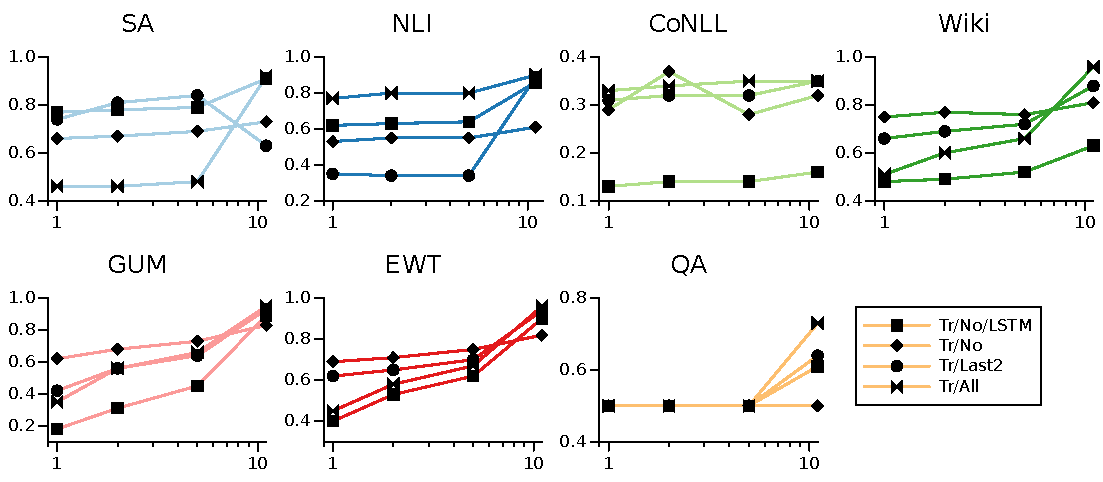
\includegraphics[width=\linewidth]{img/plot-fig2.pdf}
	\caption{\label{fig:performance-by-task} Comparison of BERT performances (macro $F_1$ score) per dataset with varying privacy budget $\varepsilon \in \{1, 2, 5, \infty \}$ on the $x$-axis (note the $\log$ scale).}
\end{figure}


\begin{tikzpicture}[overlay, remember picture]
\node at (current page.north east)[ref] {
\fullcite{senge-etal-2022-one} \par};
\end{tikzpicture}

\end{frame}


\section{DP-SGD in NLP}

\subsection{The Less Obvious Application: Language Models}

\begin{frame}{Early DP language models}

Motivated by the problem of training models for next-word prediction in a mobile keyboard; used this as a running example

\begin{tikzpicture}[overlay, remember picture]
\node at (current page.north east)[ref] {
\fullcite{McMahan.et.al.2018.ICLR} \par};
\end{tikzpicture}

\end{frame}

\begin{frame}{Early DP language models: Neighboring datasets}

Most prior work on differentially private machine learning deals with example-level privacy

--- Two datasets $D$ and $D'$ are defined to be adjacent if $D'$ can be formed by adding or removing a \textbf{single training example} from $D$

But:

--- A sensitive word or phrase may be typed several times by an individual user, but it should still be protected

\begin{tikzpicture}[overlay, remember picture]
\node at (current page.north east)[ref] {
\fullcite{McMahan.et.al.2018.ICLR} \par};
\end{tikzpicture}

\end{frame}

\begin{frame}{Early DP language models: Neighboring datasets}

\citet{McMahan.et.al.2018.ICLR} \textbf{defined}:

\begin{block}{Definition: User-adjacent datasets}
\small
Let $D$ and $D'$ be two datasets of training examples, where each example is associated with a user. Then, $D$ and $D'$ are adjacent if $D'$ can be formed by adding or removing \textbf{all of the examples associated with a single user} from $D$.
\end{block}

$D$ contains training examples, each associated with a user, e.g., $D = \{A_1, A_2, B_1, B_2\}$ where $\{A, B\}$ are the users. Then $D'$ can be formed by adding or removing all examples from one user, e.g., $D' = \{A_1, A_2\}$, or $D' = \{A_1, A_2, B_1, B_2, C_1\}$, but not $\{A_1, A_2, B_1\}$


\begin{tikzpicture}[overlay, remember picture]
\node at (current page.north east)[ref] {
\fullcite{McMahan.et.al.2018.ICLR} \par};
\end{tikzpicture}

\end{frame}


\begin{frame}{Early DP language models: Training the model with DP}

Their private algorithm relies heavily on two prior works
\begin{itemize}
\item FederatedAveraging (or FedAvg) algorithm of McMahan et al. (2016), which trains deep networks on user-partitioned data
\item the moments accountant of Abadi et al. (2016), which provides tight composition guarantees for the repeated application of the Gaussian mechanism combined with amplification-via-sampling
\end{itemize}

\begin{tikzpicture}[overlay, remember picture]
\node at (current page.north east)[ref] {
\fullcite{McMahan.et.al.2016.arXiv} \par};
\end{tikzpicture}

\end{frame}


\begin{frame}{Early DP language models: Training the model with DP}

FedAvg was introduced by McMahan et al. (2016) for federated learning, where the goal is to train a shared model while leaving the training data on each user’s mobile device. Instead, devices download the current model and compute an update by performing local computation on their dataset.

Most importantly, the algorithm naturally forms per-user updates based on a single user’s data, and these updates are then averaged to compute the final update applied to the shared model on each round.

This structure makes it possible to extend the algorithm to provide a user-level differential privacy guarantee.

\begin{tikzpicture}[overlay, remember picture]
\node at (current page.north east)[ref] {
\fullcite{McMahan.et.al.2016.arXiv} \par};
\end{tikzpicture}

\end{frame}


\begin{frame}{Early DP language models: Training the model with DP}

To achieve differential privacy:

\begin{itemize}
\item A) They use random-sized batches where we select users independently with probability $q$, rather than always selecting a fixed number of users.
\item B) They enforce clipping of per-user updates so the total update has bounded $\ell_2$ norm.
\item C) (They use different estimators for the average update)
\item D) They add Gaussian noise to the final average update.
\end{itemize}


\begin{tikzpicture}[overlay, remember picture]
\node at (current page.north east)[ref] {
\fullcite{McMahan.et.al.2018.ICLR} \par};
\end{tikzpicture}

\end{frame}


\begin{frame}{Early DP language models: Data and evaluation}

\begin{block}{Data}
\small
Used a large public dataset of Reddit posts

Each post in the database is keyed by an author, so they group the data by these keys in order to provide user-level privacy.

763,430 users each with 1600 tokens
\end{block}

\begin{block}{Evaluation}
\small
-- LSTM language model (1.35M params)

-- They evaluate using \texttt{AccuracyTop1}, the probability that the word to which the model assigns highest probability is correct
\end{block}

\begin{tikzpicture}[overlay, remember picture]
\node at (current page.north east)[ref] {
\fullcite{McMahan.et.al.2018.ICLR} \par};
\end{tikzpicture}

\end{frame}

\begin{frame}{Early DP language models: Results}

\begin{figure}
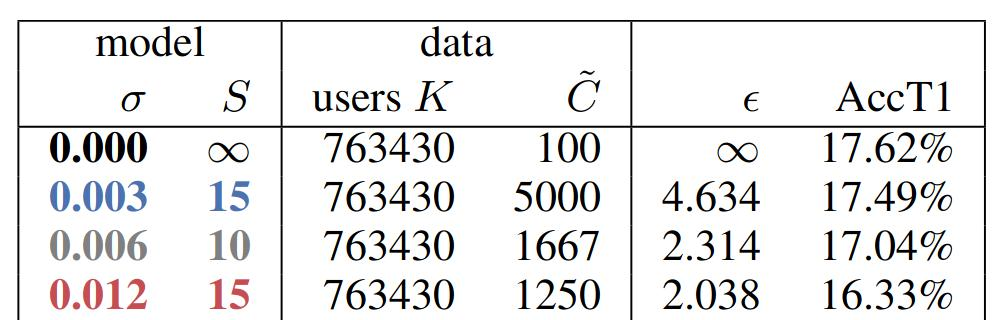
\includegraphics[width=0.8\linewidth]{img/mcmahan-table1.jpg}
\end{figure}

\begin{tikzpicture}[overlay, remember picture]
\node at (current page.north east)[ref] {
\fullcite{McMahan.et.al.2018.ICLR} \par};
\end{tikzpicture}

\end{frame}


\subsection{When Things Go Tricky}


\begin{frame}{Poisson subsampling versus just batches?}

The `standard' random shuffling method for iterating over batches providing a weaker privacy guarantee for the training data than Poisson sampling.

--- Experiments with Neural Machine Translation


\begin{tikzpicture}[overlay, remember picture]
\node at (current page.north east)[ref] {
\fullcite{igamberdiev-etal-2024-dp} \par};
\end{tikzpicture}

\end{frame}


\begin{frame}{Datasets}

--- WMT-16 (DE-EN) language pair

--- Business Scene Dialogue corpus (BSD), a collection of fictional business conversations in various scenarios (e.g. “face-to-face”, “phone call”, “meeting”), Japanese and English

--- ClinSPEn-CC, a collection of parallel COVID-19 clinical cases in English and Spanish


\begin{table}
\scriptsize
\begin{tabular}{lr|rr}
\textbf{Dataset} & \textbf{Lang. Pair} & \textbf{\texttt{\#} Trn.+Vld.} & \textbf{\texttt{\#} Test} \\
\hline
WMT-16 & DE-EN & 4,551,054 & 2,999 \\
BSD & JA-EN & 22,051 & 2,120 \\
ClinSPEn-CC & ES-EN & 1,065 & 2,870 \\  % 968 + 97
\end{tabular}
\end{table}


\begin{tikzpicture}[overlay, remember picture]
\node at (current page.north east)[ref] {
\fullcite{igamberdiev-etal-2024-dp} \par};
\end{tikzpicture}

\end{frame}


\begin{frame}{Results}

\begin{figure}
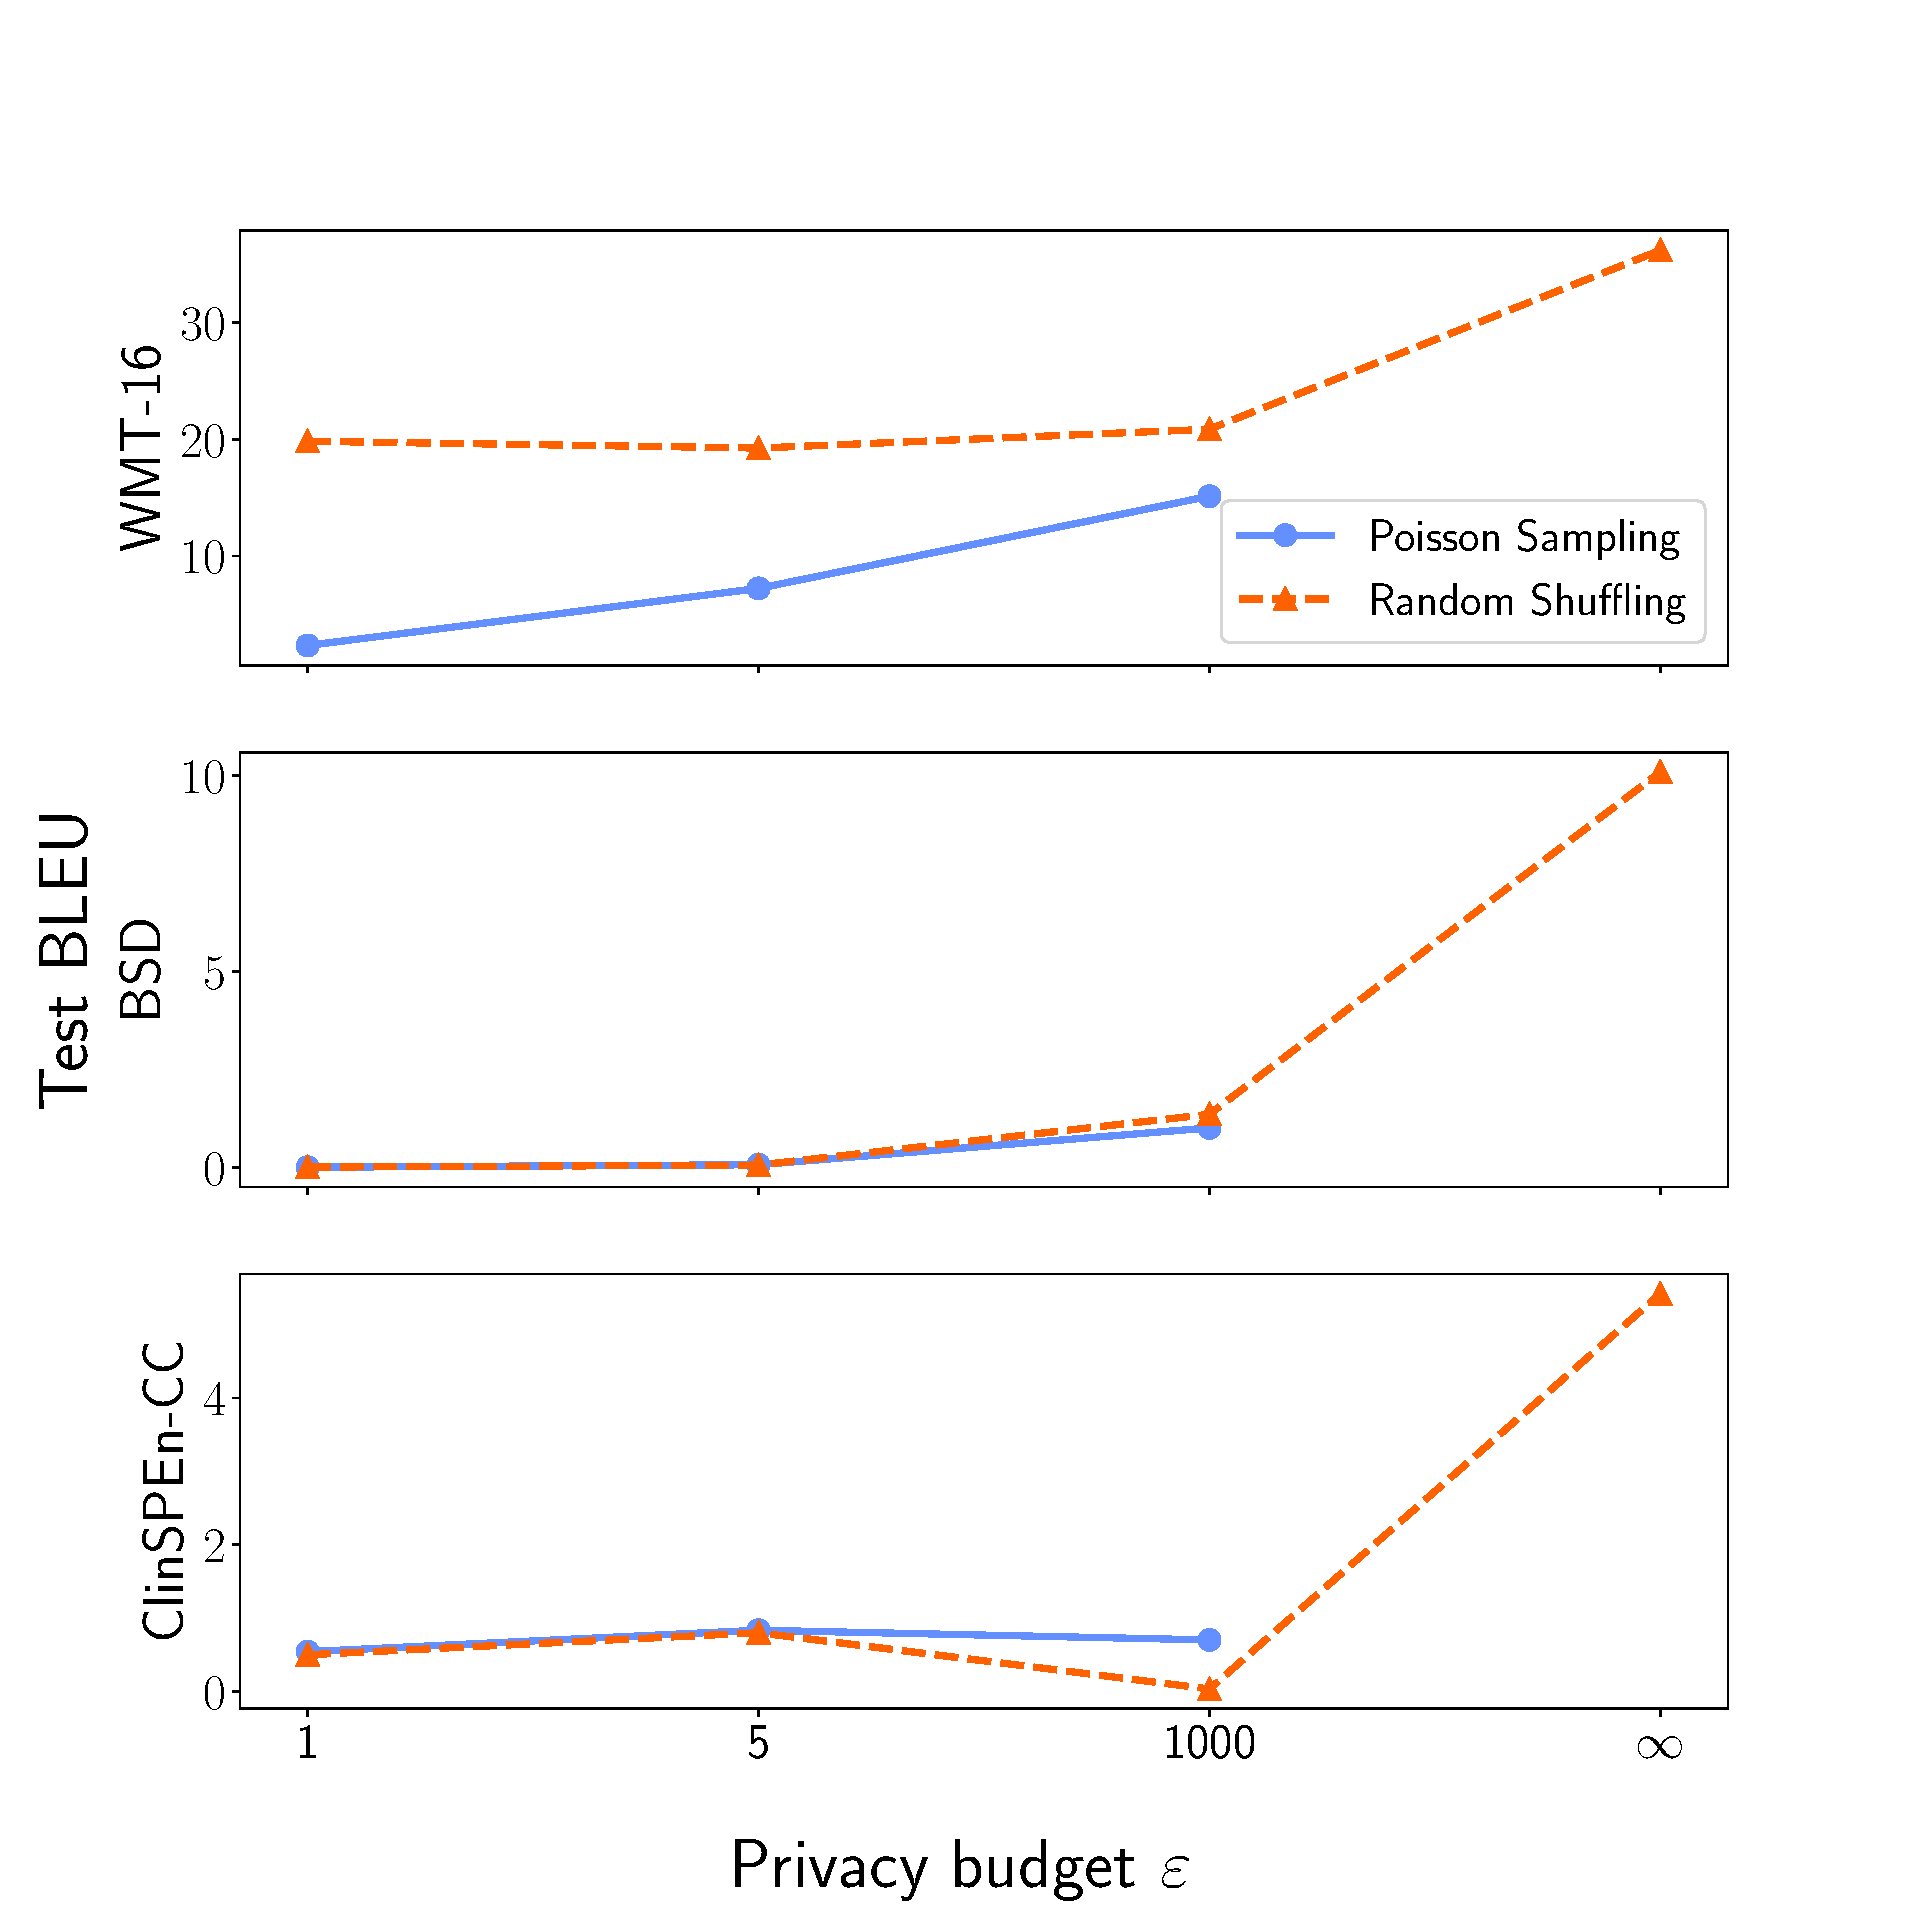
\includegraphics[trim={0 0 3cm 3.5cm},clip,width=0.6\linewidth]{img/results-test-BLEU.pdf}
\end{figure}

\begin{tikzpicture}[overlay, remember picture]
\node at (current page.north east)[ref] {
\fullcite{igamberdiev-etal-2024-dp} \par};
\end{tikzpicture}

\end{frame}



\subsection{When Things Go Very Tricky}


\begin{frame}{Private information in text?}


our understanding of what is \textit{private information} in textual data is still very limited

Applications of DP --- guarantee to each individual \textit{data point}

For textual data, a single data point will often be a sentence or document.

However, this does not mean that there is a one-to-one mapping from \textit{individuals} to sentences and documents.
For instance, multiple documents could potentially refer to the same individual, or contain the same piece of sensitive information that would break the assumption of each data point being independent.

\begin{tikzpicture}[overlay, remember picture]
\node at (current page.north east)[ref] {
\fullcite{igamberdiev-etal-2024-dp} \par};
\end{tikzpicture}

\end{frame}


\begin{frame}{Private information in text?}


``In this paper, we discuss the mismatch between the narrow assumptions made by popular data protection techniques (data sanitization and differential privacy), and the broadness of natural language and of privacy as a social norm.''


``We argue that existing protection methods cannot guarantee a generic and meaningful notion of privacy for language models. We conclude that language models should be trained on text data which was explicitly produced for public use."

\begin{tikzpicture}[overlay, remember picture]
\node at (current page.north east)[ref] {
\fullcite{Brown.et.al.2022.FAcT} \par};
\end{tikzpicture}

\end{frame}



\begin{frame}{Private information in text?}

The approach to preserving privacy in LMs has been to attempt complete removal of private information from training data (data sanitization), or to design algorithms that do not memorize private data, such as algorithms that satisfy differential privacy (DP)

Both methods make explicit and implicit assumptions about the structure of data to be protected, the nature of private information, and requirements for privacy, that do not hold for the majority of natural language data.

\begin{tikzpicture}[overlay, remember picture]
\node at (current page.north east)[ref] {
\fullcite{Brown.et.al.2022.FAcT} \par};
\end{tikzpicture}

\end{frame}



\begin{frame}{Private information in text?}

\begin{figure}
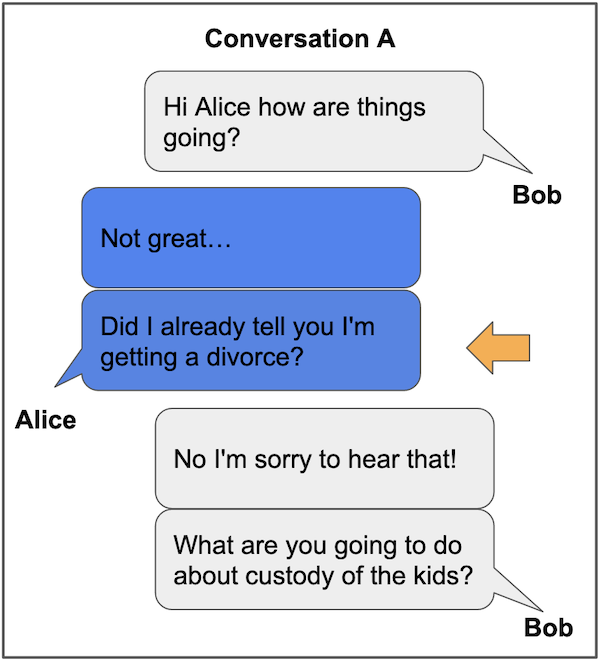
\includegraphics[width=0.45\linewidth]{img/out1.png}
\caption{Original conversation. Private information indicated by orange arrows.}
\end{figure}


\begin{tikzpicture}[overlay, remember picture]
\node at (current page.north east)[ref] {
\fullcite{Brown.et.al.2022.FAcT} \par};
\end{tikzpicture}

\end{frame}


\begin{frame}{Private information in text?}

\begin{figure}
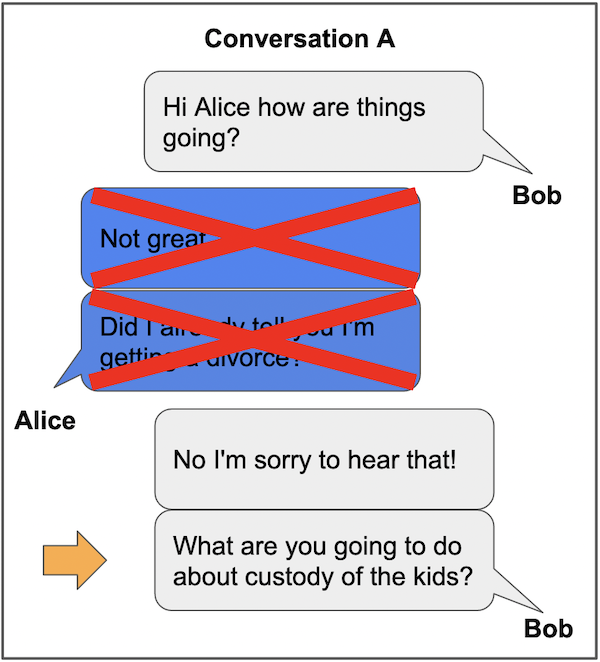
\includegraphics[width=0.45\linewidth]{img/out2.png}
\caption{Alice's messages removed. Bob's last message still includes her private information.}
\end{figure}


\begin{tikzpicture}[overlay, remember picture]
\node at (current page.north east)[ref] {
\fullcite{Brown.et.al.2022.FAcT} \par};
\end{tikzpicture}

\end{frame}


\begin{frame}{Private information in text?}

\begin{figure}
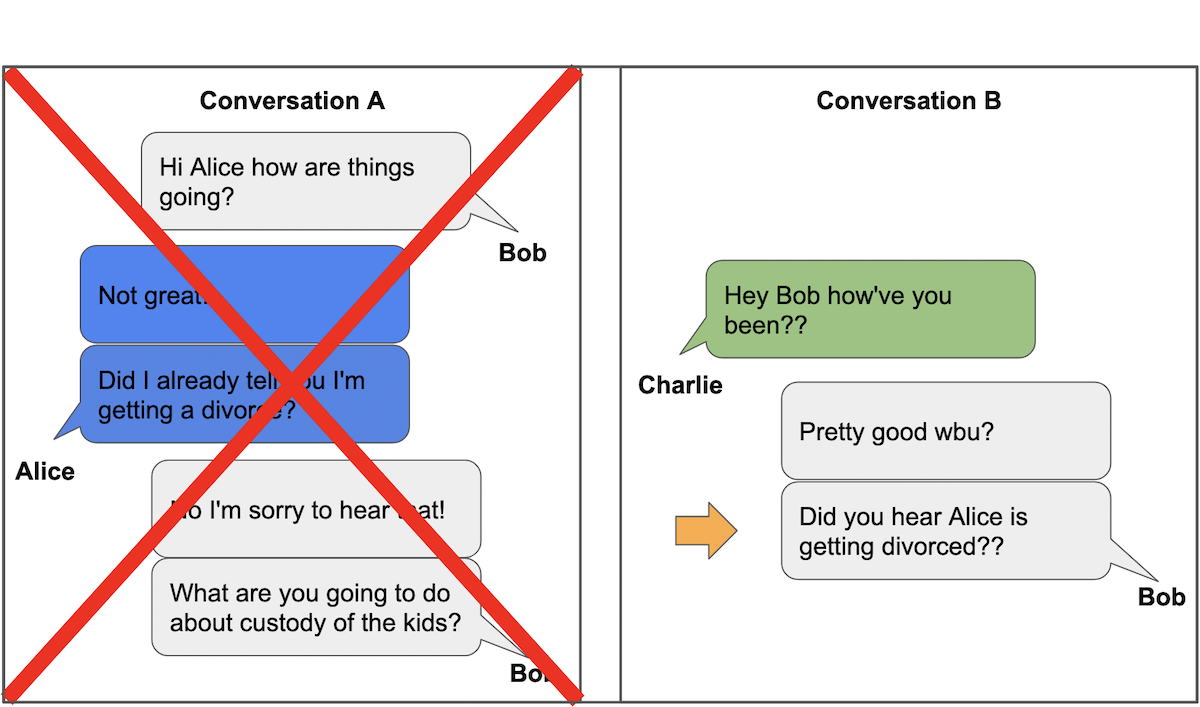
\includegraphics[width=0.75\linewidth]{img/out3.png}
\caption{The whole original conversation is removed. Conversation B still contains Alice's private information though she is not in the conversation.}
\end{figure}


\begin{tikzpicture}[overlay, remember picture]
\node at (current page.north east)[ref] {
\fullcite{Brown.et.al.2022.FAcT} \par};
\end{tikzpicture}

\end{frame}




\begin{frame}{What we covered so far}

\begin{itemize}
\item Pure $(\varepsilon, 0)$ differential privacy
\item Central and Local DP
\item Approximate $(\varepsilon, \delta)$-DP
\item Mechanisms: Laplace, Exponential, Randomized response, Gaussian
\item Post processing and composition
\item Differentially-private Stochastic Gradient Descent
\item Practical applications of DP-SGD in NLP
\end{itemize}

\end{frame}

\section{Machine unlearning}

\begin{frame}{Why machine unlearning?\footnote{
This lecture is largely based on a great blog-post by Ken Ziyu Liu, \url{https://ai.stanford.edu/~kzliu/blog/unlearning}
}}


To edit away undesired things from a (pre-trained) model, such as
\begin{itemize}
\item private data
\item stale knowledge
\item copyrighted materials
\item toxic/unsafe content, dangerous capabilities, and misinformation
\end{itemize}

\textbf{without} retraining the model from scratch


\begin{tikzpicture}[overlay, remember picture]
\node at (current page.north east)[ref] {
\fullcite{liu2024unlearning} \par};
\end{tikzpicture}

\end{frame}


\begin{frame}{What is machine unlearning?}

Removing the influences of particular training data from a trained model

Unlearning on a target model seeks to produce an \textbf{unlearned model} that is equivalent to (or at least `behaves like') a \textbf{retrained model} that is trained on the \textbf{same data} of target model, \textbf{minus} the information to be unlearned

\begin{tikzpicture}[overlay, remember picture]
\node at (current page.north east)[ref] {
\fullcite{liu2024unlearning} \par};
\end{tikzpicture}

\end{frame}

\begin{frame}{Many facets of machine unlearning}

The precise definitions of unlearning, the techniques, the guarantees, and the metrics/evaluations would depend on:

\begin{itemize}
\item The ML task (e.g., binary classification or language modeling)
\item The data to unlearn (e.g., a set of images, news articles, or the knowledge of making napalm)
\item The unlearning algorithm (e.g., heuristic fine-tuning vs deleting model components)
\item The goal of unlearning (e.g., for user privacy or harmfulness removal)
\end{itemize}

\begin{tikzpicture}[overlay, remember picture]
\node at (current page.north east)[ref] {
\fullcite{liu2024unlearning} \par};
\end{tikzpicture}

\end{frame}


\subsection{Approaches to unlearning}


\begin{frame}{Early papers on unlearning}

``To forget a piece of training data completely, systems need to revert the effects of the data on the extracted features and models."

\citet{Cao.Yang.2015.SP} coined the term \textbf{machine unlearning}

\bigskip

What would be the easiest method for unlearning?

\begin{tikzpicture}[overlay, remember picture]
\node at (current page.north east)[ref] {
\fullcite{Cao.Yang.2015.SP} \par};
\end{tikzpicture}


\end{frame}


\begin{frame}{Naive approach to unlearning}

\textbf{Retrain} the features and models \textbf{from scratch} after removing the data to be forgotten

Pros:
\begin{itemize}
\item 100\% provable: If the data points were not used for training, they cannot end up in the target model
\end{itemize}

Cons:
\begin{itemize}
\item Lack of scalability: When the training dataset is large, this approach is slow
\end{itemize}

\begin{tikzpicture}[overlay, remember picture]
\node at (current page.north east)[ref] {
\fullcite{Cao.Yang.2015.SP} \par};
\end{tikzpicture}


\end{frame}


\begin{frame}{Unlearning by \citet{Cao.Yang.2015.SP} (part 1)}

\begin{figure}
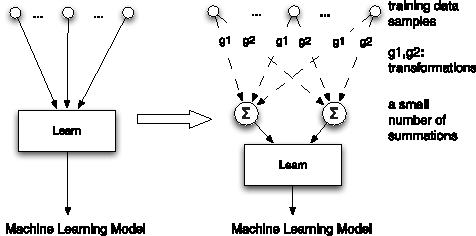
\includegraphics[width=0.4\linewidth]{img/Cao.Yang.Fig1.pdf}
\end{figure}

\begin{itemize}
\item The model consists of a small number \textbf{summations}, the learning algorithm depends only on the summations, not individual data
\end{itemize}

Unlearning: Recompute only a small number of terms, asymptotically faster than retraining from scratch


\begin{tikzpicture}[overlay, remember picture]
\node at (current page.north east)[ref] {
\fullcite{Cao.Yang.2015.SP} \par};
\end{tikzpicture}


\end{frame}


\begin{frame}{Unlearning by \citet{Cao.Yang.2015.SP} (part 2)}

\begin{figure}
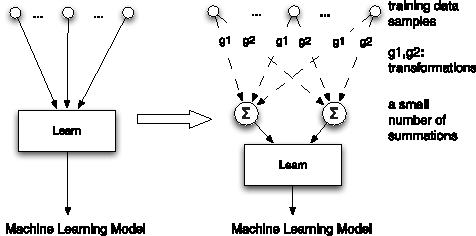
\includegraphics[width=0.4\linewidth]{img/Cao.Yang.Fig1.pdf}
\end{figure}

\begin{itemize}
\item Summations are saved together with the trained model
\item Each summation is the sum of some efficiently computable transformation of the training data samples
\end{itemize}

Unlearning: Recompute only a small number of terms, asymptotically faster than retraining from scratch


\begin{tikzpicture}[overlay, remember picture]
\node at (current page.north east)[ref] {
\fullcite{Cao.Yang.2015.SP} \par};
\end{tikzpicture}


\end{frame}


\begin{frame}{Limitations of unlearning by \citet{Cao.Yang.2015.SP}}

\begin{itemize}
\item Algorithm limited to very structured problems only \citep{Sekhari.et.al.2021.NeurIPS}
\end{itemize}

\begin{tikzpicture}[overlay, remember picture]
\node at (current page.north east)[ref] {
\fullcite{Sekhari.et.al.2021.NeurIPS} \par};
\end{tikzpicture}


\end{frame}



\subsection{Sharded, Isolated, Sliced, and Aggregated (SISA) training}

\begin{frame}{Unlearning versus Differential Privacy}

ML models potentially memorize training data $\to$ important to unlearn what they have learned from data to be deleted.

\begin{itemize}
\item Enforcing $\varepsilon$-differential privacy with $\varepsilon \neq 0$ does \textbf{not} alleviate the need for an unlearning mechanism
\item While DP algorithms guarantee a bound on how much individual training points contribute to the model, there is a \textbf{non-zero} contribution from each point (if this was not the case, the model would not be able to learn at all)
\end{itemize}

We require that a point has \textbf{no influence} on the model once it has been unlearned

\begin{tikzpicture}[overlay, remember picture]
\node at (current page.north east)[ref] {
\fullcite{Bourtoule.et.al.2021.SP} \par};
\end{tikzpicture}


\end{frame}



\begin{frame}

\begin{figure}
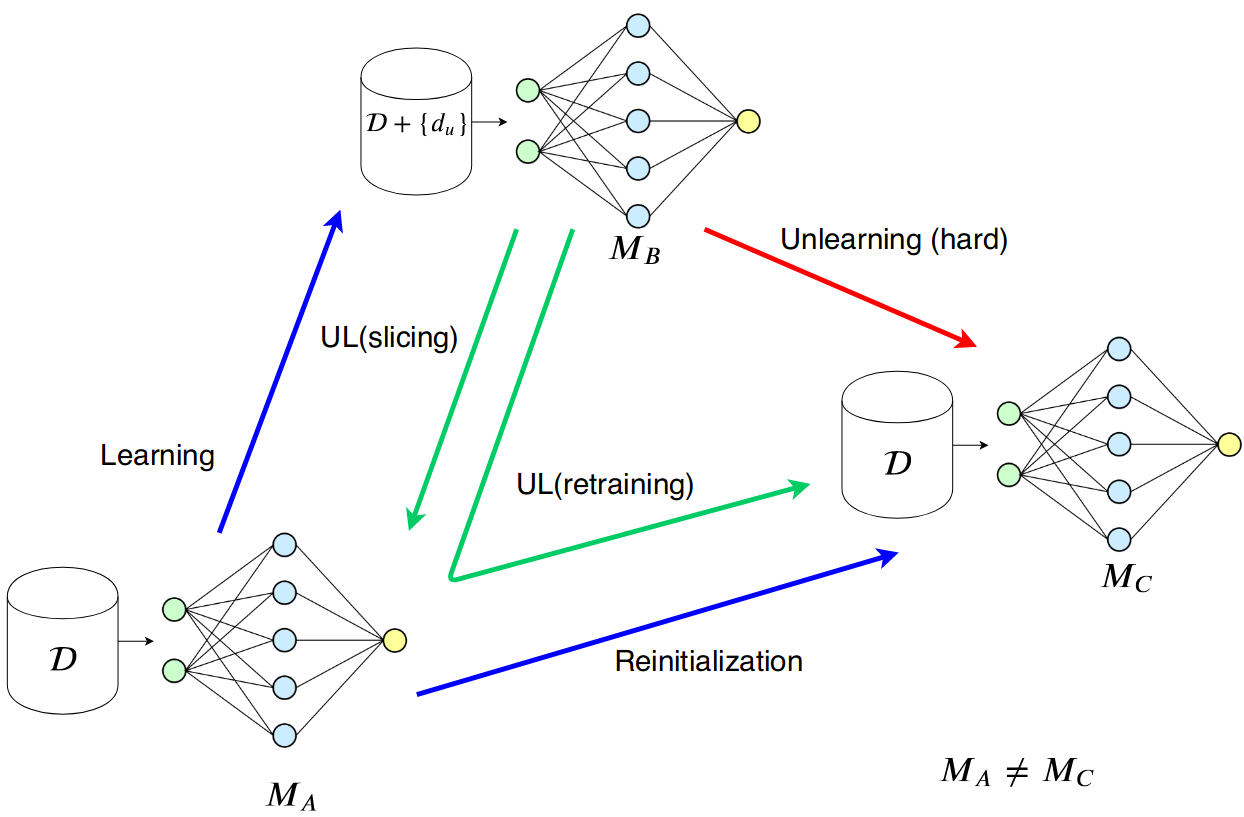
\includegraphics[width=0.85\linewidth]{img/unlearning1.png}	
\end{figure}
\vspace{-1.4em}
\small{
Unlearning (red arrow) is hard because there exists no function that measures the influence of augmenting the dataset $\mathcal{D}$ with point $d_u$ and fine-tuning a model $M_A$ already trained on $\mathcal{D}$ to train (left blue arrow) a model $M_B$ for $\mathcal{D} + \{d_u\}$.
}

\begin{tikzpicture}[overlay, remember picture]
\node at (current page.north east)[ref] {
\fullcite{Bourtoule.et.al.2021.SP} \par};
\end{tikzpicture}


\end{frame}



\begin{frame}

\begin{figure}
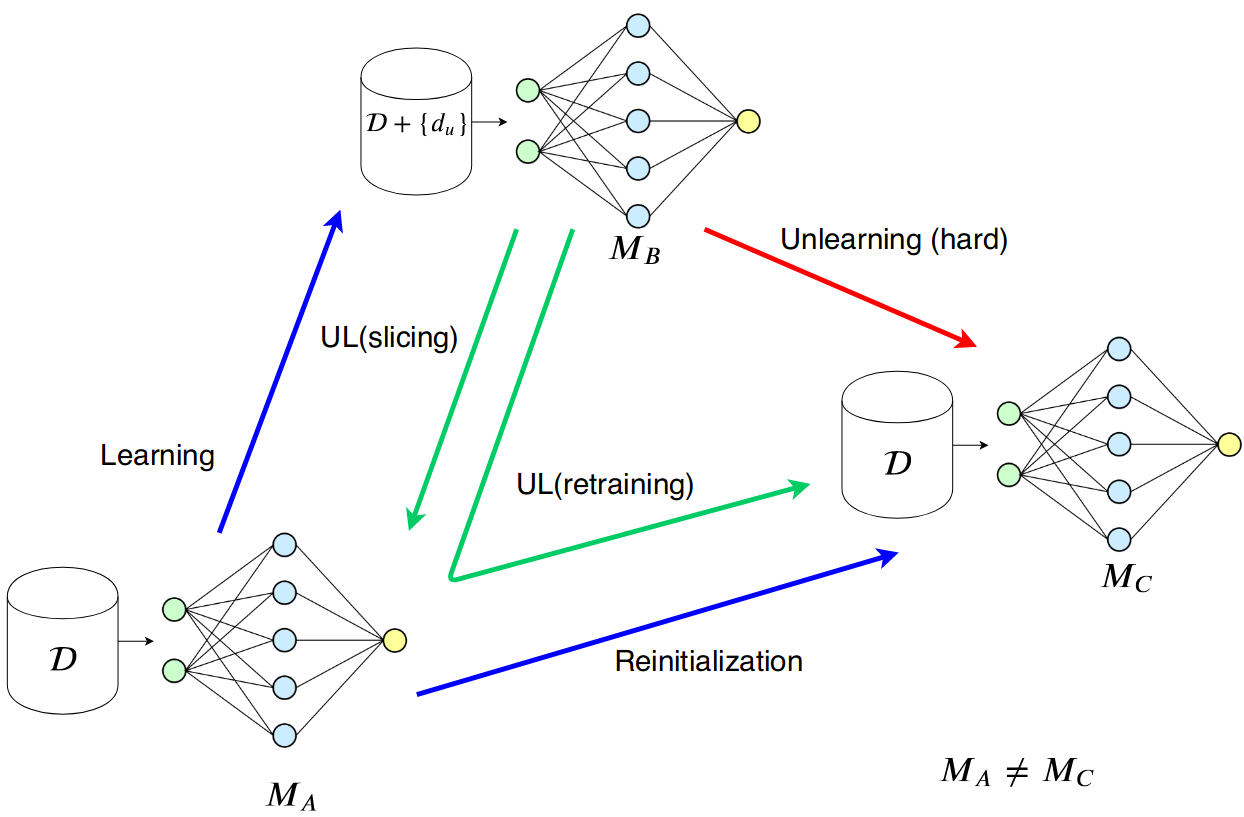
\includegraphics[width=0.7\linewidth]{img/unlearning1.png}	
\end{figure}
\vspace{-1.3em}
\small{
This makes it impossible to revert to model $M_A$ without saving its parameter state before learning about $d_u$. We call this model slicing (short green arrow). In the absence of slicing, one must retrain (curved green arrow) the model without $d_u$, resulting in a model $M_C$ that is different from the original model $M_A$.
}

\begin{tikzpicture}[overlay, remember picture]
\node at (current page.north east)[ref] {
\fullcite{Bourtoule.et.al.2021.SP} \par};
\end{tikzpicture}


\end{frame}



\begin{frame}{SISA training approach}

Retraining from scratch while omitting data points that need to be unlearned: most straightforward way, provable guarantees

SISA training replicates the model being learned several times where each replica receives a disjoint shard (or subset) of the dataset—similar to current distributed training strategies. We refer to each replica as a constituent model.

SISA training deviates from other strategies: there is no flow of information between constituent models

\begin{tikzpicture}[overlay, remember picture]
\node at (current page.north east)[ref] {
\fullcite{Bourtoule.et.al.2021.SP} \par};
\end{tikzpicture}


\end{frame}

\begin{frame}{SISA training approach (contd.)}

Each shard is further partitioned into slices, where each constituent model is trained incrementally (and iteratively, in a stateful manner) with an increasing number of slices.

At inference, the test point is fed to each constituent and all the constituents’ responses are aggregated, similar to the case of ML ensembles


When a data point is to be unlearned, only the constituent model whose dataset contains this point is affected

\begin{tikzpicture}[overlay, remember picture]
\node at (current page.north east)[ref] {
\fullcite{Bourtoule.et.al.2021.SP} \par};
\end{tikzpicture}


\end{frame}



\begin{frame}{SISA training approach (contd.)}

Sharding is possible for any model or hypothesis class: it has no impact on how training is performed beyond the smaller set of data each model has access to


Slicing is possible for any iterative learning algorithm that is stateful: the algorithm should be such that it can continue to learn from its current state when presented with new data. Gradient descent naturally falls under that category

\begin{tikzpicture}[overlay, remember picture]
\node at (current page.north east)[ref] {
\fullcite{Bourtoule.et.al.2021.SP} \par};
\end{tikzpicture}


\end{frame}




\begin{frame}{SISA training approach (contd.)}

\begin{figure}
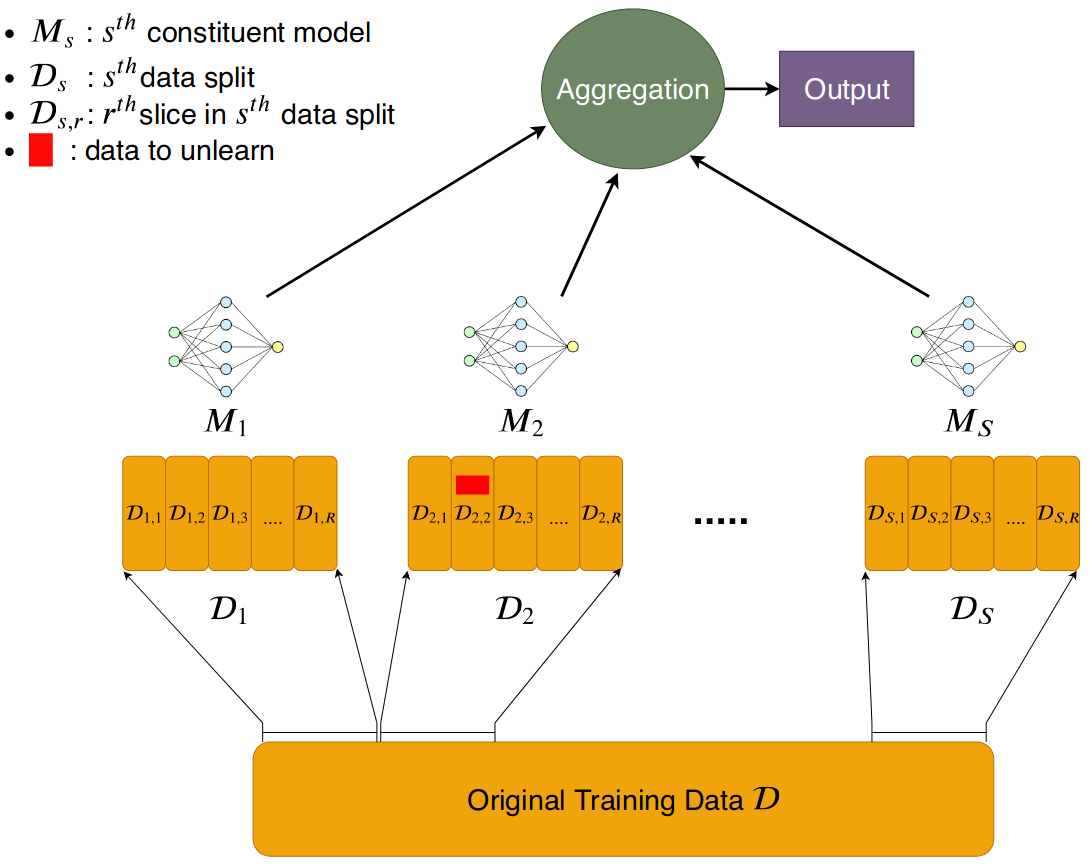
\includegraphics[width=0.7\linewidth]{img/unlearning2.png}
\end{figure}

\begin{tikzpicture}[overlay, remember picture]
\node at (current page.north east)[ref] {
\fullcite{Bourtoule.et.al.2021.SP} \par};
\end{tikzpicture}


\end{frame}



\begin{frame}{SISA inference and testing}

Inference: a voting strategy where each constituent contributes equally to the final outcome through a simple label-based majority vote

\bigskip

SISA framework tested on more than a million images; typical speed improvements ranged from 2.45 to 4.63-times for unlearning tasks \citep{Greengard.2022.ACM}

\begin{tikzpicture}[overlay, remember picture]
\node at (current page.north east)[ref] {
\fullcite{Greengard.2022.ACM} \par};
\end{tikzpicture}


\end{frame}


\begin{frame}{SISA limitations}

While the SISA concept is promising, it has limitations:

\begin{itemize}
\item For example, by reducing the amount of data per shard, there is an impact on machine learning and a lower-quality outcome is likely
\end{itemize}

\begin{tikzpicture}[overlay, remember picture]
\node at (current page.north east)[ref] {
\fullcite{Greengard.2022.ACM} \par};
\end{tikzpicture}


\end{frame}



\begin{frame}{SISA limitations}


SISA = model checkpointing, in which the learner \textbf{preemptively stores backup models} in which certain points have been excluded

\begin{itemize}
\item This strategy makes it easy to quickly return an appropriate backup model upon receiving a deletion request
\item The downside is that one typically has to store a number of additional models which scales with the training data size, which may be \textbf{prohibitively large}
\end{itemize}


\begin{tikzpicture}[overlay, remember picture]
\node at (current page.north east)[ref] {
\fullcite{Sekhari.et.al.2021.NeurIPS} \par};
\end{tikzpicture}


\end{frame}



\subsection{Unlearning with probabilistic theoretical guarantees}

\begin{frame}{Unlearning without storing the original data}

Suppose a learning algorithm $A$ over dataset $S$ outputs the model $A(S)$

An unlearning algorithm $\bar{A}$ takes as input the model $A(S)$ and a set $U \subseteq S$ of data samples that are to be deleted, and is required to output a new model $\tilde{w}$

The unlearning algorithm $\bar{A}$ can also access some additional data statistics $T(S)$
$$
\bar{A}(U, A(S), T(S)) \mapsto \tilde{w} \in W
$$
The unlearning algorithm does not have access to the entire original dataset $S$ and hence cannot retrain from scratch

\begin{tikzpicture}[overlay, remember picture]
\node at (current page.north east)[ref] {
\fullcite{Sekhari.et.al.2021.NeurIPS} \par};
\end{tikzpicture}

\end{frame}


\begin{frame}{Formalizing unlearning}

$\bar{A}(U, A(S), T(S)) \mapsto \tilde{w} \in W$

Probability of the unlearning algorithm outputting a certain unlearned model:
$$
\Pr(\bar{A}(U, A(S), T(S)) \in W)
$$

$S \setminus U$ is the original dataset $S$ after removing samples to be unlearned $U$


Probability of the unlearning algorithm outputting a certain unlearned model (but this time the original model and statistics were trained on $S \setminus U$):
$$
\Pr(\bar{A}(\emptyset, A(S \setminus U), T(S \setminus U)) \in W)
$$

\begin{tikzpicture}[overlay, remember picture]
\node at (current page.north east)[ref] {
\fullcite{Sekhari.et.al.2021.NeurIPS} \par};
\end{tikzpicture}

\end{frame}


\begin{frame}{$\varepsilon, \delta$-unlearning by \citet{Sekhari.et.al.2021.NeurIPS}}

For $0 \leq \varepsilon \leq 1$ and $\delta > 0$:
$$
\begin{aligned}
\Pr(\bar{A}(U, A(S), T(S)) \in W) &\leq \exp(\varepsilon) \cdot \\
&\Pr(\bar{A}(\emptyset, A(S \setminus U), T(S \setminus U)) \in W) \\ 
&+ \delta
\end{aligned}
$$
and
$$
\begin{aligned}
\Pr(\bar{A}(\emptyset, A(S \setminus U), T(S \setminus U)) \in W) &\leq \exp(\varepsilon) \cdot \\
&\Pr(\bar{A}(U, A(S), T(S)) \in W) \\ 
&+ \delta
\end{aligned}
$$

The above states that with high probability, an observer cannot differentiate between the two cases

\begin{tikzpicture}[overlay, remember picture]
\node at (current page.north east)[ref] {
\fullcite{Sekhari.et.al.2021.NeurIPS} \par};
\end{tikzpicture}

\end{frame}


\begin{frame}{$\varepsilon, \delta$-unlearning by \citet{Sekhari.et.al.2021.NeurIPS}}

Retraining from scratch would mean
$$
\bar{A}(U, A(S), T(S)) = A(S \setminus U)
$$
but it would require $T(S)$ contain the entire dataset $S$

\bigskip

Summary:
\citet{Sekhari.et.al.2021.NeurIPS} proposed an unlearning algorithm for convex loss functions

\begin{tikzpicture}[overlay, remember picture]
\node at (current page.north east)[ref] {
\fullcite{Sekhari.et.al.2021.NeurIPS} \par};
\end{tikzpicture}

\end{frame}


\subsection{Examples of Machine Unlearning in NLP}


\begin{frame}{Adapting SISA}
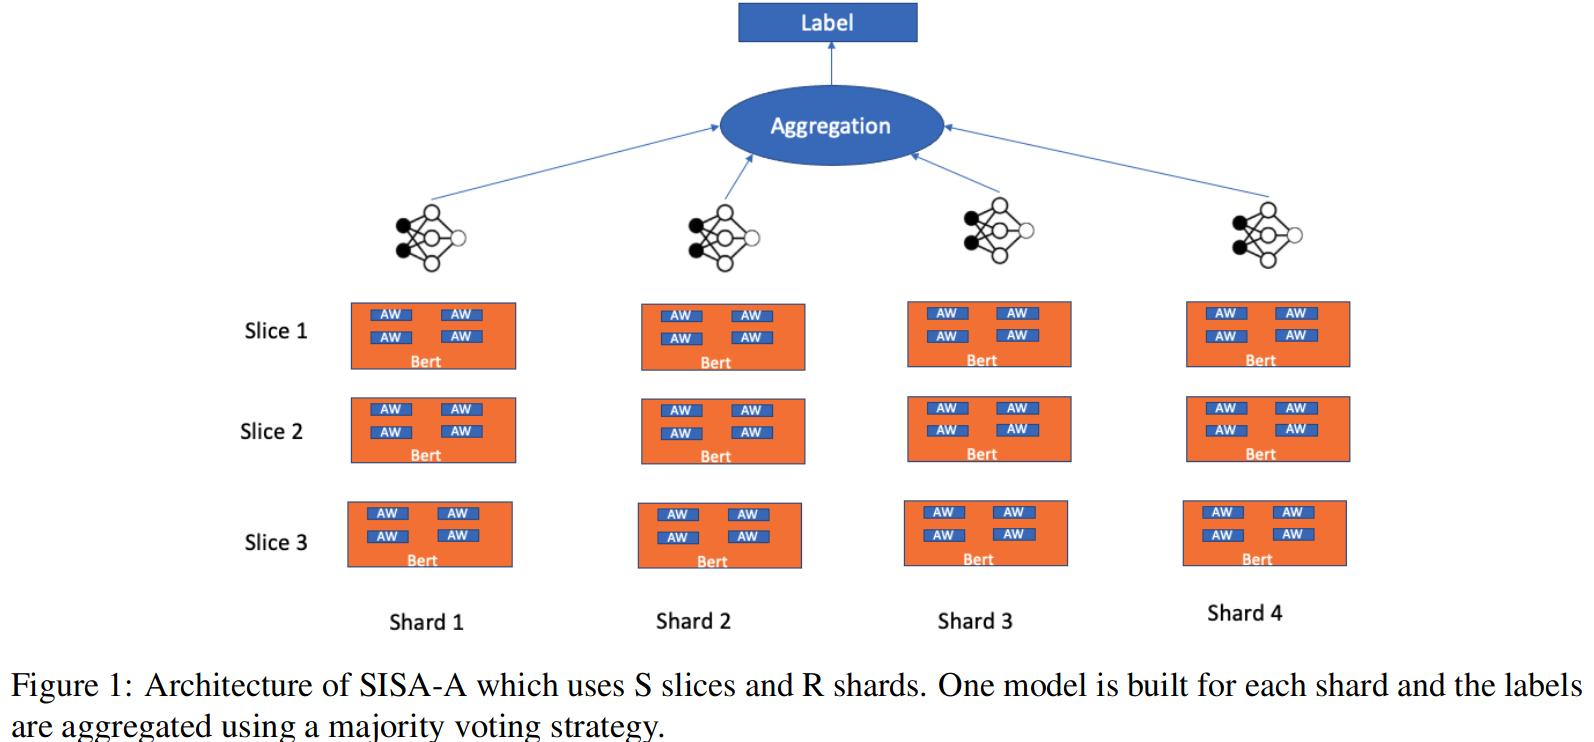
\includegraphics[width=\linewidth]{img/sisa-bert.jpg}


The model goes through the data, slice by slice saving a checkpoint after training for each slice in each shard

\begin{tikzpicture}[overlay, remember picture]
\node at (current page.north east)[ref] {
\fullcite{Bannihattikumar.et.al.2023.FindingsAACL} \par};
\end{tikzpicture}

\end{frame}


\begin{frame}{Adapting SISA}
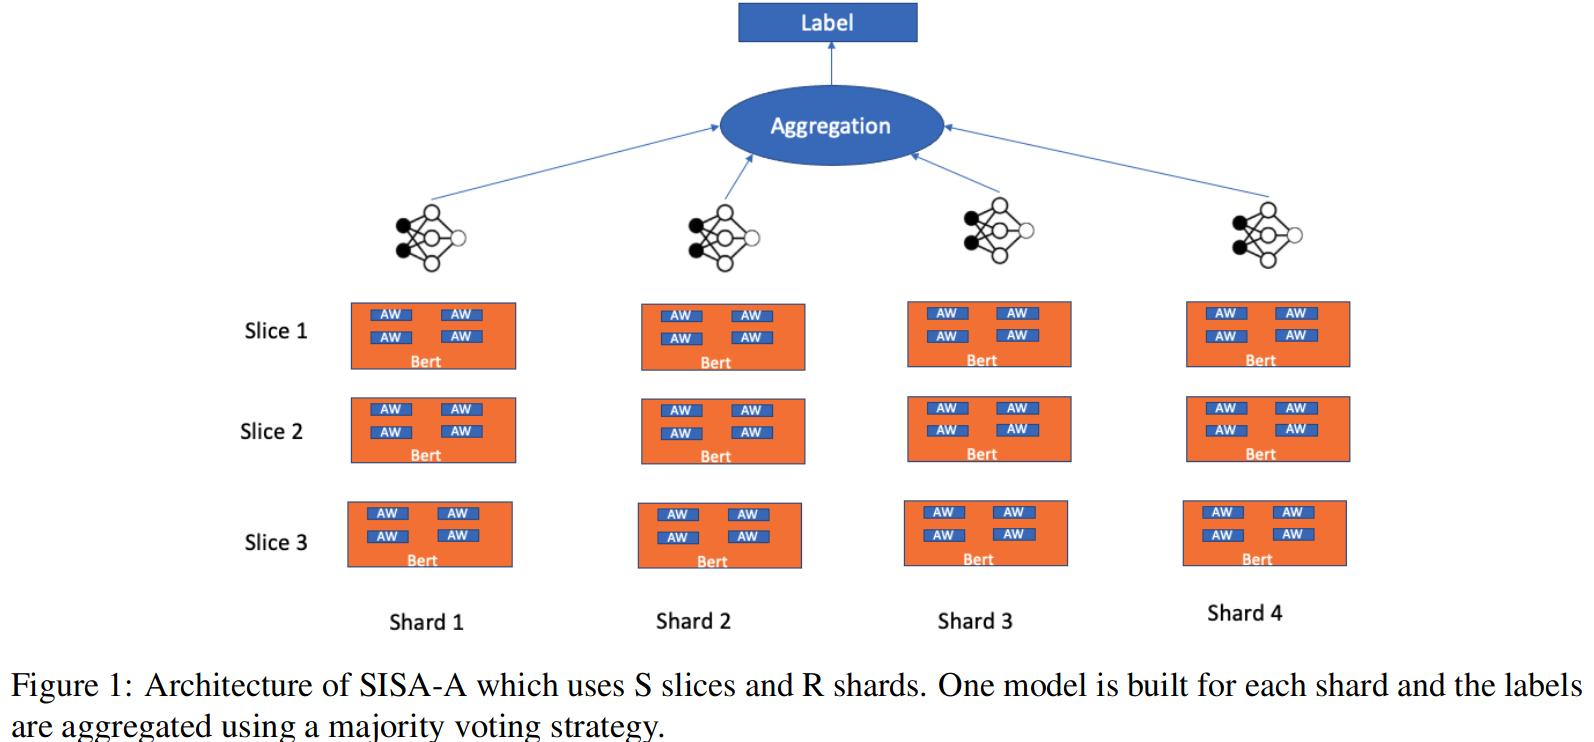
\includegraphics[width=0.7\linewidth]{img/sisa-bert.jpg}

Un-learning request: pick the shard and the slide where this data point is present

Delete the datapoint from this slice, take the previous checkpoint, continue training

\begin{tikzpicture}[overlay, remember picture]
\node at (current page.north east)[ref] {
\fullcite{Bannihattikumar.et.al.2023.FindingsAACL} \par};
\end{tikzpicture}

\end{frame}



\begin{frame}{Adapting SISA: Choice of checkpoints}

SISA-FC
\begin{itemize}
\item Fine-tune only the final fully-connected (FC) layers of BERT
\end{itemize}

Adapters \citep{Houlsby.et.al.2019.ICML}
\begin{itemize}
\item Adapters in the Encoder blocks of the transformer. This increases the memory footprint of the model, it only accounts for about 1--5\% of the model parameters (95--99\% memory benefits)
\end{itemize}




\begin{tikzpicture}[overlay, remember picture]
\node at (current page.north east)[ref] {
\fullcite{Bannihattikumar.et.al.2023.FindingsAACL} \newline \fullcite{Houlsby.et.al.2019.ICML} \par};
\end{tikzpicture}

\end{frame}


\begin{frame}{Another approach to unlearning in transformers}

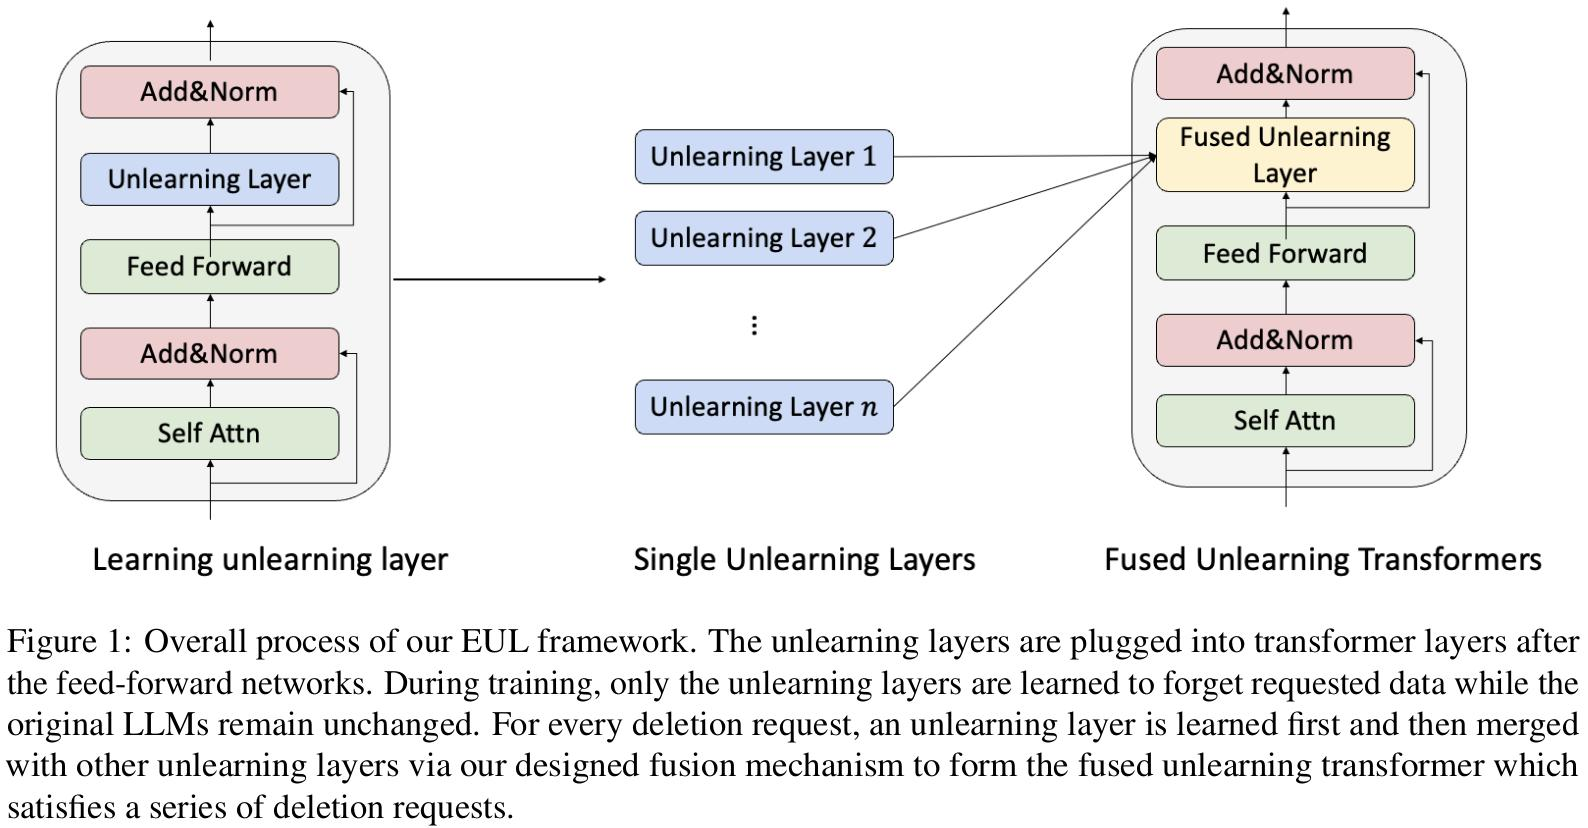
\includegraphics[width=\linewidth]{img/unlearning-emnlp.jpg}

\begin{tikzpicture}[overlay, remember picture]
\node at (current page.north east)[ref] {
\fullcite{Chen.Yang.2023.EMNLP} \par};
\end{tikzpicture}

\end{frame}





\begin{frame}{License and credits}

	\begin{columns}
		\begin{column}{0.7\textwidth}
			Licensed under Creative Commons Attribution-ShareAlike 4.0 International (CC BY-SA 4.0)
		\end{column}
		\begin{column}{0.2\textwidth}
			
\includegraphics[width=0.9\linewidth]{img/cc-by-sa-icon.pdf}
		\end{column}
	\end{columns}
	
	\bigskip
	
	Credits
	
	\begin{scriptsize}
		
		Ivan Habernal
		
		Content from ACL Anthology papers licensed under CC-BY \url{https://www.aclweb.org/anthology}
		
		Partly inspired by lectures from Gautam Kamath
	
	\end{scriptsize}
	
\end{frame}



\end{document}

